\section{Results} 
\subsection{descriptive statistics}
The summary presented in Table \ref{tab:table3} and histogram in Fig \ref{fig:boxplots-all} show a better understanding of the energy consumption data of web apps. 

\begin{table}[h!]
  \begin{center}
    \begin{tabular}{l|r} % <-- Alignments: 1st column left, 2nd middle and 3rd right, with vertical lines in between
      \textbf{  } & \textbf{Energy consumption} \\
      \hline
      Min & 3.543\\
      1st Qu. & 71.025\\
      Median & 153.555\\
      Mean & 480.398 \\
      3rd Qu. & 362.120 \\
      Max & 9820.064 \\
      St. deviation & 1080.97\\
    \end{tabular}
        \caption{Summary energy consumption.}
           \label{tab:table3}
  \end{center}
\end{table}



The energy consumption is between 3.543 joules and 9820.064 joules. The central tendency based on the median lies around 153.555 joules. Using the skewness formula \cite{Rep:e1071}, we are able to quantify the skewness of the data. We tested for skewness and achieved a result of 4.77. This value demonstrates a positive skewness as values that deviate from zero implies that the data is not symmetrical. This is further corroborated by the shape of Fig. \ref{fig:boxplots-all}, with the data showing a long tail towards the higher energy consumption values. A standard deviation of 1080.97 joules shows that there is a big spread in the data. We zoomed in on the energy consumption per level in Fig. \ref{fig:boxecv} and Fig. \ref{fig:scatpvsec}. We created energy consumption box-plots diagrams and scatter-plots for the performance levels Good, Average and Poor.


\begin{figure}[H]
  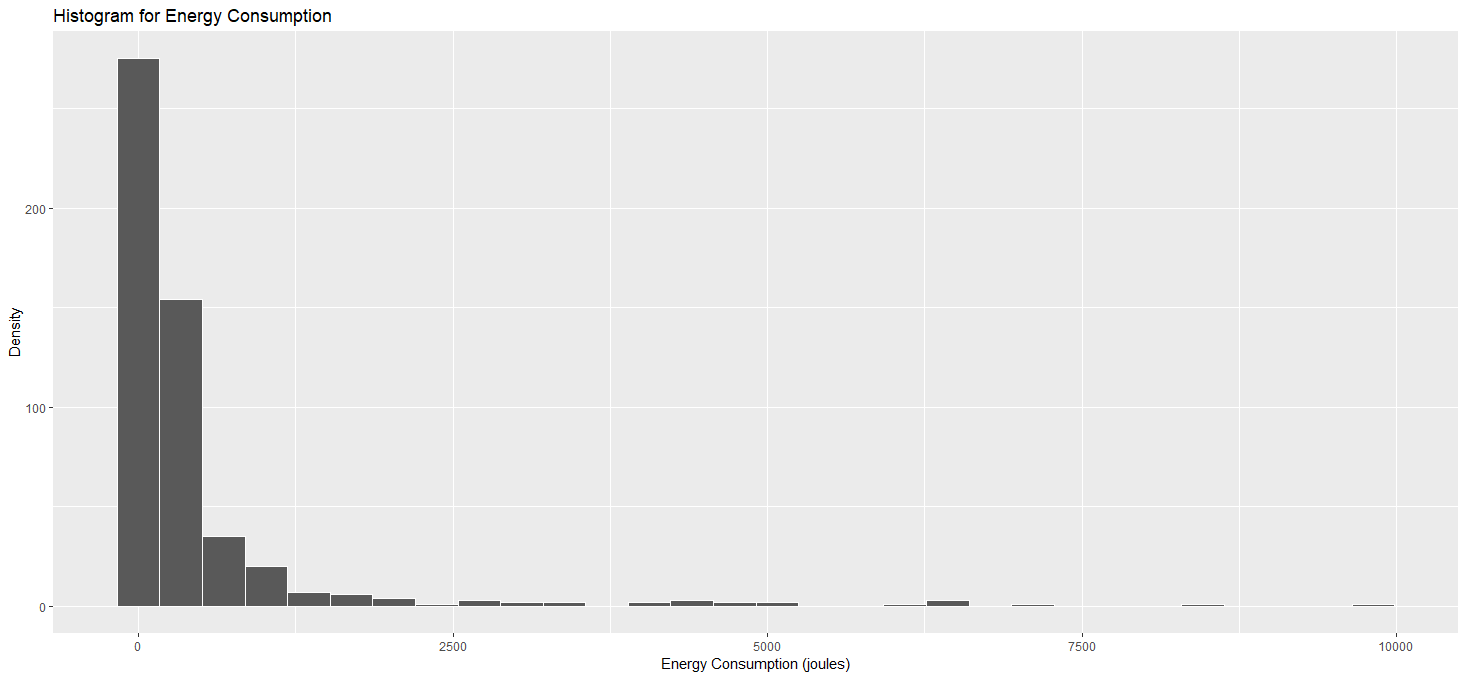
\includegraphics[width=\linewidth]{./NewImages/Fig_4_Histogram_Energy_Consumption.png}
  \caption{Histogram energy consumption}
  \label{fig:histec}
\end{figure}



\begin{figure}[H]
  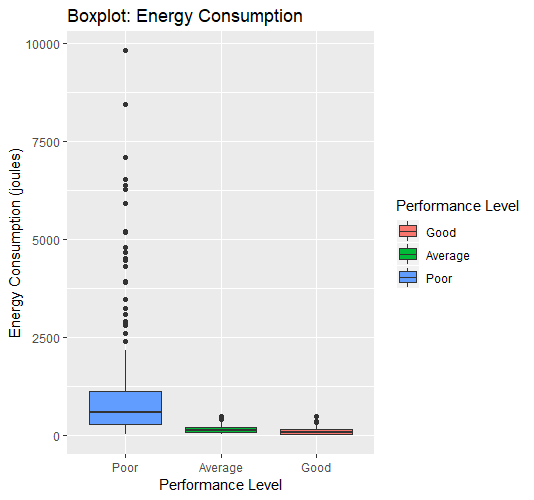
\includegraphics[width=\linewidth]{./NewImages/Fig_5_Box_Plot_Energy_Per_Level.png}
  \caption{Box-plot energy consumption per treatment}
  \label{fig:boxecv}
\end{figure}

\begin{figure}[H]
  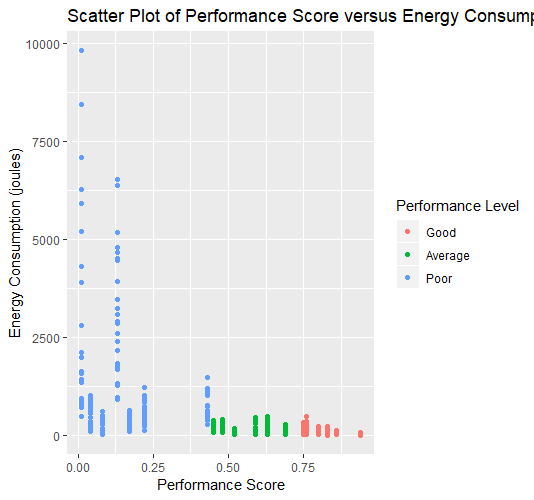
\includegraphics[width=\linewidth]{./NewImages/Fig_6_Scatterplot_Perf_score_Energy.png}
  \caption{Scatter-plot performance vs energy consumption}
  \label{fig:scatpvsec}
\end{figure}

From the diagrams, we could see that the energy consumption measurements for Good and Average are pretty similar; both of these groups are centered around the same energy consumption value, and their outliers are quite similar. Comparing both the good and average performance values to the Poor performance level, we see a bigger difference. The median energy consumption from poor performing web apps is higher when compared to good and average performance web apps. \newline

The histogram for energy consumption in Fig. \ref{fig:histec} indicates that the energy consumption data is not normal. To justify our assumption we performed a Q-Q plot against a random sample of the normal distribution in Fig. \ref{fig:qqec}.

\begin{figure}[H]
  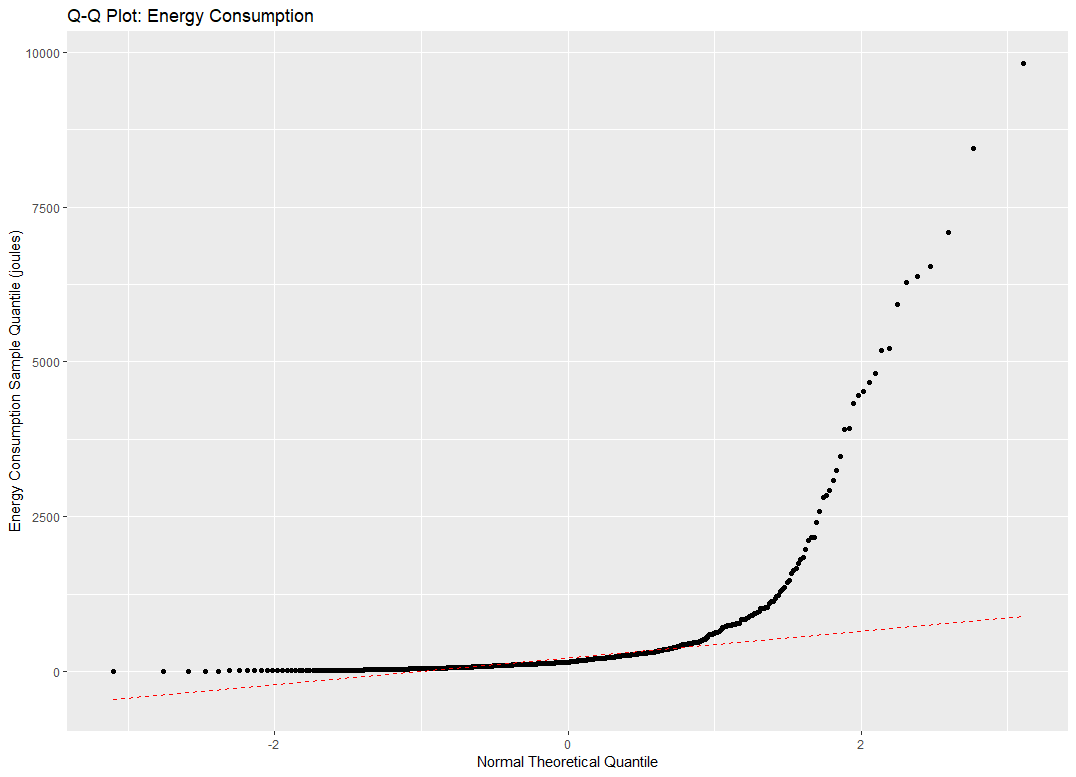
\includegraphics[width=\linewidth]{./NewImages/Fig_7_QQPLOT_RAW.png}
  \caption{Q-Q-plot energy consumption}
  \label{fig:qqec}
\end{figure}

The assumption of non normality for the energy consumption data could be caused by the rather small sample size of 21 web apps, or extreme values caused by the distortion of the data. We would prefer to use parametric statistics based on the higher statistical power of these tests. We performed various data transformations on the energy consumption data, including the squared (Fig. \ref{fig:histqq-sqr}), reciprocal (Fig. \ref{fig:histqq-rec}), and the log transformation of the collected data (Fig. \ref{fig:histqq-log}). The most promising transformation is the log operation on the energy consumption sample:

\begin{figure}[H]
  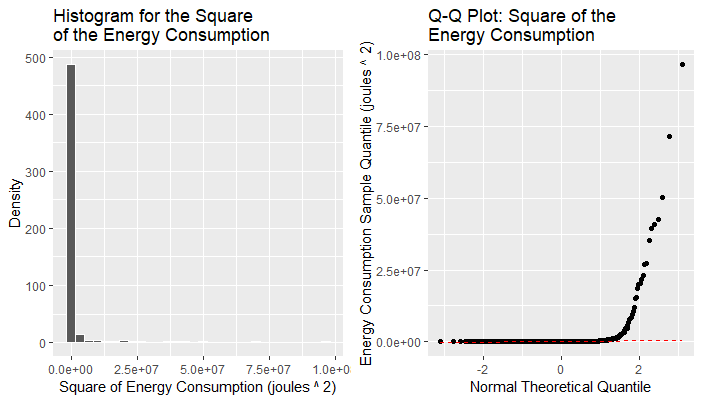
\includegraphics[width=\linewidth]{./NewImages/Fig_8_Squared_Transform.png}
  \caption{Squared transformation for energy consumption}
  \label{fig:histqq-sqr}
\end{figure}

The square transformation of the energy consumption exacerbated the skewness of the data to a skewness value of 8.311, and this is clearly seen from both the histogram and the Q-Q plot.  The Histogram does not show the characteristic bell-shape of normal data and the Q-Q plot demonstrates a more pronounced curvature.


\begin{figure}[H]
  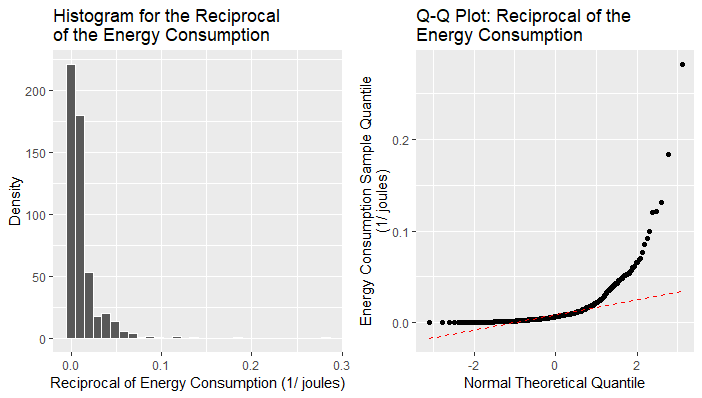
\includegraphics[width=\linewidth]{./NewImages/Fig_9_Reciprocal_Transform.png}
  \caption{Reciprocal transformation for energy consumption}
  \label{fig:histqq-rec}
\end{figure}

The reciprocal transformation was able to better approximate our data to a normal distribution. Skewness decreased to a value of 5.736. However, the curvature of the Q-Q plot is still quite pronounced.

\begin{figure}[H]
  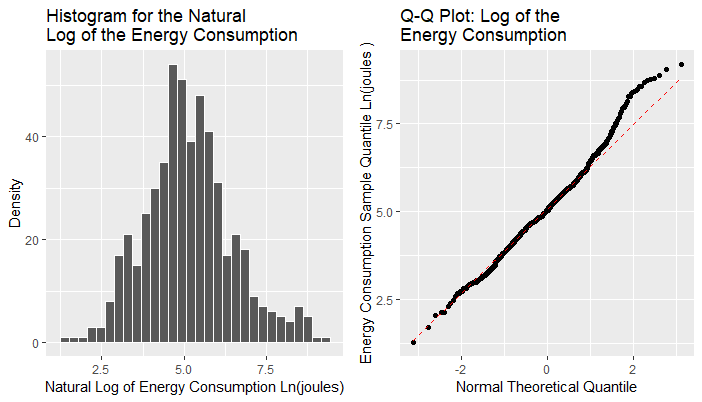
\includegraphics[width=\linewidth]{./NewImages/Fig_10_Log_Transform.png}
  \caption{Log transformation for energy consumption}
  \label{fig:histqq-log}
\end{figure}

We check the histogram of the log of the data, and we see that the skewness is dramatically improved. However the data is still positively skewed with an estimated value of 0.353, and the Quantile-Quantile plot shows a slight curvature. Furthermore, we performed the Shapiro - Wilks test, and received a p-value of 2.89e-4, thus there exists evidence to deny the null hypothesis that the transformed data lies within the normal distribution.


\subsection{Hypothesis testing}
As the assumption that the data comes from a normal distribution was not met, we performed the Kruskal Wallis non-parametric test based on our experiment design. 
The Kruskal Wallis rank based non-parametric test is used to determine if there are statistically significant differences between the energy consumptions at the different treatment levels: Good, Average, Poor. Employing the grouping technique from Lighthouse ensures a representative design, given that the performance scores themselves are defined in relation to the scores of other web apps.

In order to perform the test we made a numeric vector for our treatment levels by using a value of 3 for high performing web apps whereas a value of 1 for poor performance level. We got a p-value of 2.2e-16. Therefore, we can reject the null hypothesis that the means of energy consumption for each performance levels are equal.

Then we checked the correlation between the performance score of a web app and its energy consumption by using the spearman non-parametric correlation test. We obtained a negative correlation value of -0.664 for energy consumption with respect to performance, which infers that the energy consumption increases as the level of performance drops. 

After that we performed a post-hoc pairwise comparison using Dunn tests due to the non-parametric nature of the data. Given that multiple pairwise comparisons are performed, the p-value must be corrected to avoid the higher probability of getting statistically significant results by chance.  We used the Bonferroni correction technique for the pairwise comparison test. We got a p-value of 9.371e-52 for comparison between good and poor and a p-value of 3.534e-27 between average and poor performance levels. This results show that  there is significant difference between good versus poor and average versus poor performance levels. Between Good and average, we got a p-value of 1.226e-4.  Thus, there exists evidence for all pairwise comparisons that their distributions are different from each other. 

Next we applied Cliff's delta to investigate the effect size. Effect size will help us to know the quantified measure of the difference between two groups as it emphasizes more on the size of the difference rather than mixing it up with sample size. By looking at the delta estimate of -0.336  we found that the effect size is medium when comparing good and average levels. For the comparison between good-poor and average-poor we get delta estimates of -0.857 and -0.768 respectively. These results show that the effect size for those treatment levels is large.

\begin{figure}[H]
  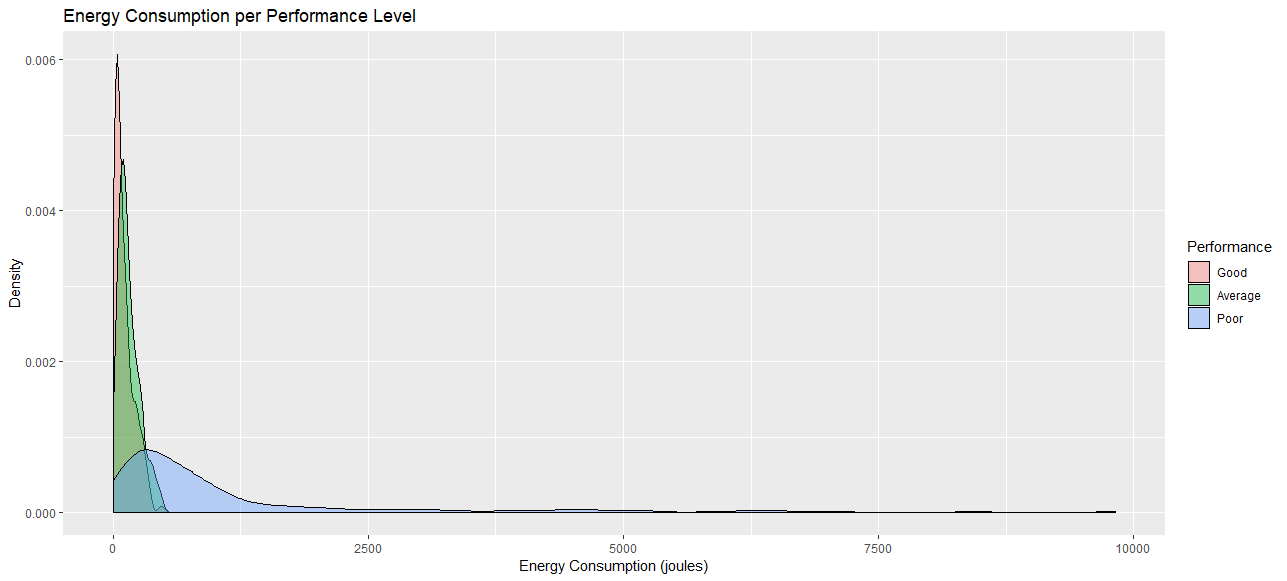
\includegraphics[width=\linewidth]{./NewImages/Fig_11_Density_Curve_Energy_Consumption.png}
  \caption{Density curve for energy consumption}
  \label{fig:density-levels}
\end{figure}

In order to support the results given by Cliff's delta test we depicted in Fig. \ref{fig:density-levels} a density graph with different levels. In this graph we can see that the differences in density between all the performance levels are significant.  However,  the difference in density between good and average performance levels is less than the difference when comparing to poor performance web apps.  
